\pdfminorversion=3
\documentclass[tikz]{standalone}
\usepackage{schemabloc}
%\usepackage{vuiprepstandalone}
%\usepackage{alain2}

\begin{document}
\footnotesize

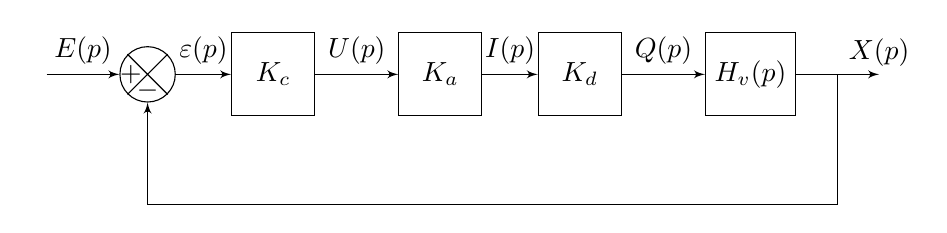
\begin{tikzpicture}
\sbEntree{E}

\sbComp{c1}{E}
    \sbRelier[$E(p)$]{E}{c1}

\sbBloc{b1}{$K_c$}{c1}
    \sbRelier[$\varepsilon(p)$]{c1}{b1}

\sbBloc[3]{b2}{$K_a$}{b1}
    \sbRelier[$U(p)$]{b1}{b2}

\sbBloc{b3}{$K_d$}{b2}
    \sbRelier[$I(p)$]{b2}{b3}

\sbBloc[3]{b4}{$H_v(p)$}{b3}
    \sbRelier[$Q(p)$]{b3}{b4}

\sbSortie[3]{S}{b4}
    \sbRelier{b4}{S}
    \sbNomLien[0.8]{S}{$X(p)$}

%\sbDecaleNoeudy[4]{S}{n1} 
%\sbDecaleNoeudx[-2]{n1}{n2} 
%\sbBlocr{r}{$G(p)$}{n2} 
%\sbRelieryx{b1-S}{r}
%\sbRelierxy[$R(p)$]{r}{c1}

\sbRenvoi{b4-S}{c1}{}

%\draw [latex-] (c2) --++ (0,1) node[left] {$\text{Pert}(p)$};

\end{tikzpicture}

\normalsize
\end{document}